\documentclass[12pt, a4paper]{article}

% Use reasonably small margins
\usepackage{fullpage}

% for various math utilities
\usepackage{amsmath}
\usepackage{amssymb}
\usepackage{commath}
\usepackage{cancel}
\usepackage{breqn}
\usepackage{fancyhdr}
\usepackage{tcolorbox}
\usepackage{blindtext} 
\usepackage{ragged2e}
\usepackage{tocloft}
\usepackage{tikz}
\usetikzlibrary{calc}
\usepackage{enumitem}
\usepackage{parskip}
\newcommand\HRule{\rule{\textwidth}{1pt}}


\headsep = 40pt
\footskip = 40pt
\textheight = 600pt
\headheight = 15pt
\pagestyle{fancy}
\fancyhf{}
\rhead{\thepage}
\lhead{Project 2013-2017}
\lfoot{Dept. of Computer Science and Engineering}
\renewcommand{\headrulewidth}{1pt}
\renewcommand{\footrulewidth}{1pt}
\renewcommand{\contentsname}{\hfill\hfill \bfseries\LARGE CONTENTS\hfill \vspace*{1cm}}  
\renewcommand{\cftaftertoctitle}{\hfill}
\renewcommand{\cftdot}{}
\usepackage[colorlinks=true,linkcolor=black]{hyperref}
% provides non-italicized Greek letters in text
\usepackage[euler]{textgreek}

% provides the \includegraphics command
\usepackage{graphicx}
\usepackage{subfig}

% allows figure environments to be placed in exact locations
\usepackage{float}

% Bold caption labels, and give captions increased margins
\usepackage[labelfont=bf, margin=1cm]{caption}

% allows for configurable source code listings
\usepackage{listings}
\usepackage{color}
\definecolor{dkgreen}{rgb}{0,0.6,0}
\definecolor{gray}{rgb}{0.5,0.5,0.5}
\definecolor{red}{rgb}{0.8,0,0}
\hypersetup{linktocpage}
\lstset{frame=tb,
  language=C,
  aboveskip=3mm,
  belowskip=3mm,
  showstringspaces=false,
  columns=flexible,
  basicstyle={\small\ttfamily},
  numbers=left,                    % where to put the line-numbers; possible values are (none, left, right)
  numbersep=5pt,                   % how far the line-numbers are from the code
  numberstyle=\tiny\color{gray}, % the style that is used for the line-numbers
  stepnumber=1,                    % the step between two line-numbers. If it's 1, each line will be numbered
  keywordstyle=\color{blue},
  commentstyle=\color{dkgreen},
  stringstyle=\color{red},
  breaklines=true,
  breakatwhitespace=true,
  breakindent=50pt,
  tabsize=4
}

\DeclareMathOperator*{\argmin}{arg\,min\:}

\begin{document}

\begin{titlepage}

\begin{tikzpicture} [overlay,remember picture]
       \draw [line width=1mm ,yellow!50!red] 
        ($ (current page.north west) + (1cm, -1cm) $)
        rectangle
        ($ (current page.south east) + (-1cm,1cm) $);

\end{tikzpicture}

\begin{tikzpicture} [overlay,remember picture]
       \draw [line width=0.3mm,orange ] 
        ($ (current page.north west) + (11.5mm, -11.5mm) $)
        rectangle
        ($ (current page.south east) + (-11.5mm,11.5mm) $);

\end{tikzpicture}
\begin{center}
\vspace*{-3cm}
\textcolor{red!40!orange}{\Large \bfseries N.S.S. COLLEGE OF ENGINEERING} \\[5mm]
\textcolor{red!40!orange}{\large \bfseries PALAKKAD, KERALA - 678008 } \\[1cm]
{\fontsize{5mm}{1mm}\bfseries UNIVERSITY OF CALICUT } \\[2mm]
\begin{figure}[ht!]
    \centering
    
\includegraphics[width=15cm,height=4cm,keepaspectratio]{nss3.png}
\end{figure}
\textcolor{red!40!orange}{\fontsize{13pt}{1pt}  \textbf{DEPARTMENT OF COMPUTER SCIENCE AND ENGINEERING}}\\[1cm]

{\normalsize \textbf{ PROJECT REPORT \\ 2013-2017}}\\[0.8cm]
  {\Large \textbf{MOBILE DATA SERVERS USING }}\\[0.2cm]
    {\Large \textbf{ ANDROID SYSTEMS}}\\[0.5cm]
\textcolor{red!40!orange}{\fontsize{13pt}{1pt}  \textbf{SUBMITTED BY}}\\[5mm]
\hspace{15mm}
\begin{minipage}{.366\textwidth}
\textbf{AKASH G KRISHNAN}\\[2mm]
\textbf{BINEESH P B}\\[2mm]
\textbf{DIVYA P}\\[2mm]
\textbf{HARIKRISHNAN R}\\[2mm]
\textbf{RAHEESA MUMTHAZ V}\\
\end{minipage}
\begin{minipage}{.2\textwidth}
\textbf{NSANECS005}\\[2mm]
\textbf{NSANECS017}\\[2mm]
\textbf{NSANECS020}\\[2mm]
\textbf{NSANECS023}\\[2mm]
\textbf{NSANECS041}\\
\end{minipage}
\newline
\vspace*{1mm}

\textcolor{red!40!orange}{\fontsize{13pt}{1pt}  \textbf{GUIDED BY}}\\[2mm]
{\normalsize \textbf{Mrs. CHITRA S NAIR}}\\[1mm]
{\normalsize \textbf{Assistant Professor}}\\[1mm]
{\normalsize \textbf{Dept. of Computer Science and Engineering}}\\[1mm]
{\normalsize \textbf{N.S.S.C.E, Palakkad}}\\[2mm]

\end{center}
\end{titlepage}
\newpage
\begin{titlepage}

\begin{tikzpicture} [overlay,remember picture]
       \draw [line width=1mm ,yellow!50!red] 
        ($ (current page.north west) + (1cm, -1cm) $)
        rectangle
        ($ (current page.south east) + (-1cm,1cm) $);

\end{tikzpicture}

\begin{tikzpicture} [overlay,remember picture]
       \draw [line width=0.3mm,orange ] 
        ($ (current page.north west) + (11.5mm, -11.5mm) $)
        rectangle
        ($ (current page.south east) + (-11.5mm,11.5mm) $);

\end{tikzpicture}
\begin{center}
\vspace*{-3cm}
\textcolor{red!40!orange}{\Large \bfseries N.S.S. COLLEGE OF ENGINEERING} \\[5mm]
\textcolor{red!40!orange}{\large \bfseries PALAKKAD, KERALA - 678008 } \\[1cm]
{\fontsize{5mm}{1mm}\bfseries UNIVERSITY OF CALICUT } \\[2mm]
\begin{figure}[ht!]
    \centering
    
\includegraphics[width=15cm,height=4cm,keepaspectratio]{nss3.png}
\end{figure}
\textcolor{red!40!orange}{\fontsize{13pt}{1pt}  \textbf{DEPARTMENT OF COMPUTER SCIENCE AND ENGINEERING}}\\[1cm]
\textcolor{red!40!orange}{\normalsize  \textbf{CERTIFICATE}}\\[5mm]
\justify
\hspace{3cm}This \hspace{0.2mm}is \hspace{0.2mm} to \hspace{0.2mm} certify \hspace{0.2mm} that \hspace{0.2mm} this \hspace{0.2mm} is \hspace{0.2mm} the  \hspace{0.2mm} bonafide \hspace{0.2mm} report \hspace{0.2mm} of  \hspace{0.2mm}the \hspace{0.2mm} \hspace{0.2mm} Project entitled  \hspace{2mm}\textbf{MOBILE  \hspace{0.5mm} DATA \hspace{0.5mm} SERVERS  \hspace{0.5mm}USING  \hspace{0.5mm}ANDROID  \hspace{0.5mm} SYSTEMS} \hspace{2mm} done by
\textbf{AKASH G KRISHNAN, BINEESH P B, DIVYA P, HARIKRISHNAN R, RAHEESA MUMTHAZ V }  in partial fulfillment of the requirements for the award of the Degree of Bachelor of Technology in Computer Science and Engineering under University of Calicut.\\[1.6cm]
\hspace*{10mm}
\begin{minipage}{.55\textwidth}
\textcolor{red!40!orange}{\normalsize  \textbf{GUIDED BY}}\\[5mm]
{\normalsize \textbf{ CHITRA S NAIR}}\\
{\normalsize \textbf{ Assistant Professor}}\\
\hspace*{-8mm}{\normalsize \textbf{Dept. of Computer Science \\and Engineering}}\\[1.5cm]
\textcolor{red!40!orange}{\normalsize  \textbf{STAFF IN CHARGE}}\\[5mm]
{\normalsize \textbf{ANURAJ MOHAN}}\\
{\normalsize \textbf{ Assistant Professor}}\\
\hspace*{-8mm}{\normalsize \textbf{Dept. of Computer Science \\ and Engineering}}\\
\end{minipage}
\begin{minipage}{.6\textwidth}
\vspace*{-36.5mm} 
\hspace*{-5mm}\textcolor{red!40!orange}{\normalsize  \textbf{HEAD OF DEPARTMENT}}\\[5mm]
{\hspace*{-5mm}\normalsize \textbf{VIJI RAJENDRAN V}}\\[-0.5mm]
\hspace*{-2mm}{\normalsize \textbf{ Associate Professor}}\\[0.5mm]
\hspace*{-8mm}{\normalsize \textbf{Dept. of Computer Science \\and Engineering}}\\[1cm]
\end{minipage}
\end{center}
\end{titlepage}
\newpage
%--------------------------------------------------
% INTRODUCTION TO POSITIONING
%--------------------------------------------------

\begin{center}
{\huge \bfseries ACKNOWLEDGEMENT} \\[3cm]
\end{center}
Many noble hearts contributed immense inspiration and technical assistance for the successful completion of our project work. We are unable to express our gratitude in words to such individuals. 
\\

\hspace{5mm}First of all, we thank the Almighty \textbf{God}, for granting us the strength, courage and knowledge to complete this project successfully. 
We acknowledge our sincere thanks to the management of N.S.S College of Engineering for their help in the successful completion of the project. We would also like to express our deep regard to our principal\\ \textbf{Prof. T SUDHA} for helping us  complete the project successfully. 
\\

\hspace{5mm}We take this opportunity to express our profound gratitude to our Head of  the  \\Department, \textbf{Assoc.Prof. VIJI RAJENDRAN V} and project head, \textbf{Asst.Prof. ANURAJ MOHAN} for all their valuable support towards making the project a grant success.We take this opportunity to express our profound gratitude to our project guide, \textbf{Asst.Prof.  CHITRA S NAIR},  for all her guidance and valuable support towards making our project a grant success. 
\\

\hspace{5mm}We are also thankful to our teachers, \textbf{Mr.Balagopal N}, \textbf{Mrs.Sindhu S },  \textbf{Mrs.Sruthy Manmadhan}, \textbf{Mr.Pillai Praveen Thulasidharan}, \textbf{Mr. Kiran V K }and \textbf{Mr. Syam Sankar}  for their valuable guidance throughout our project.We would also like to thank all the non-teaching staff of our department for their constant encouragement throughout our project. Last, but not the least, we take pleasant privilege in expressing our heart full thanks to our friends who were of precious help in completing our project.
\newpage


\begin{center}
{\huge \bfseries SYNOPSIS} \\[3cm]
\end{center}
Most of the data in the current internet was created in the last two years with the enormous number of selfies and other datas being created every second. It is not near that the time will come when we run out of space to store the data that is created. Our project aims to help solve this problem to a bit. The project  convert the existing mobile phones into small data servers which can be used to store enormous amount of data.

\hspace{5mm}If this is implemented,  it would help in increasing the space to store the data without increasing web servers.  This can also affect the economy since there will be a huge change in the cost of maintaining servers. The servers setup can be used to store data such as images or other documents without increasing the server spaces. Distributed data servers, can be created on mobile phones by implementing NoSQL. 

\hspace{5mm}Multiple phones or nodes can be interlinked and connected to a main server, in order to make distributed database management possible in the case of mobile phones. That is, Local databases which can store data like text can be created on mobile phones using this technique. 

\hspace{5mm}If a person requires a particular file, he can request for it to the server, which can be a local server or a server on the internet. If it is a local server, we can connect to it directly,through wifi or other networks. If using a server on internet, we will connect to it using the internet. 

\hspace{5mm}This technique can be used to request the mobile phone users around the world, to allocate some space from their phone memory for creating servers. In the present condition websites like Facebook, Instagram have large storage servers, and have to maintain huge servers. This requires wholesome amounts spend on their maintenance and control every year. But if this technology of distributed data servers is developed, only very crucial data need to be stored in the main server of these websites. Other files e can be encrypted and distributively stored in the millions of phones around the globe.



\newpage

\tableofcontents
\listoffigures
\vfill
\newpage

%--------------------------------------------------
% INTRODUCTION TO POSITIONING
%--------------------------------------------------
\begin{center}
\section{INTRODUCTION}\vspace{5mm}
\end{center}
There are more than 1 billion people who are using smart phones in this world. I'm There are more than 3 billion mobile phones around the world. Every day new mobile applications are developed and most of them need internet connection to work. The databases have been the most common way of storing and managing data. A million people use the internet to search for information online every second. These information are stored in servers that are spread across the world. \\

\subsection{Motivation}
\hspace{5mm}As the amount of data on internet is increasing day by day, the storage should also needs to be increased. This causes the creation and maintenance of huge data servers which leads to several problems like pollution, massive power usage etc. This project is to convert the existing mobile phones into Data servers which can store enormous amount of data. This if implemented, can revolutionize the web servers since there will be a huge change in the cost of maintaining servers. The servers setup can be used by open source services like Wikipedia to store data. Distributed data servers, can be created on mobile phones by implementing NoSQL.
\\
\subsection{Problem Definition}
\hspace{5mm}The use of internet is becoming more popular day by day leads to a requirement of a mass storage for the data. Everyone is using mobile phone storage and other secondary devices to store the data, but prefer to have a backup in cloud so that the data will not be lost and can be accessed whenever needed. So this leads to the requirement of large data servers and maintaining the severs. The setup and maintenance cost for the same is also very high. Also environmental pollution due to this is also high. So considering the economic and environmental difficulties,the proposed system will make use of the storage in existing mobile phones which is now available in large numbers.
\subsection{Objective}
\begin{itemize}
\item Utilise the storage  resources of mobile devices.
\end{itemize}
\hspace{10mm}Nowadays we are having a large number of mobile phones all around the world.If this storage resource is efficiently utilised,many problems regarding creation and maintenance of huge data servers can be resolved.

\begin{itemize}
\item Decrease number of existing servers.
\end{itemize}
\hspace{10mm}If mobile phones can be used to store the data,the number of servers can also be reduced that will produce a great impact on decreasing pollution due to data servers.

\begin{itemize}
\item Efficient utilization of existing Servers.
\end{itemize}
\hspace{10mm}If mobile phones are used as data servers which will leads to the efficient usage of existing servers so that adding more servers will no more required.This will create a great economical advantage.

\begin{itemize}
\item Lower power consumption.
\end{itemize}
\hspace{10mm}Since mobile phones are very common and its power consumption is less compared to servers,storage of data and maintenance will be easier than that in data servers.

\begin{itemize}
\item Lower pollution 
\end{itemize}
\hspace{10mm}Internet makes everyday transactions very easier and efficient.But the amount of pollution it creates is much higher.Especially from servers,the amount of greenhouse gases emitted is very high and therefore it creates a lot of problems to the surroundings.
Data centres are the second most power-hungry elements of the internet.The amount of heat exhausted from the servers is also very large as power consumption.Reports show that 90 percentage of energy is simply wasted. So switching to mobile data servers will help to decrease the pollution.
\\

\hspace{5mm}In present world people view information in websites. But most of these information are stored in large servers that pollute the environment.The database is a common method of storing data. There are different relational databases like Oracle DB by Oracle, MSSQL by Microsoft ,MySQL is an open source database by Oracle etc. There is another type of Database called NoSQL which is something not similar to Relational Databases. Some of them are MongoDB , CoughBase etc . There are also databases inside the mobile devices. The commonly used database on mobiles is SQLite.
\\

\hspace{5mm} SQLite is a small version of the SQL that was originally developed for the web. It uses less space to store data. But it has some disadvantages similar to that of SQL which was solved using NoSQL in web. We here try to use the NoSQL concept into smart phones and solve some of the issues of SQLite using NoSQL .The NoSQL we have used here is Snappy DB. Snappy DB is a NoSQL database based on Level DB developed by Google and use snappy compression to compress the data stored in it .
\\

\hspace{5mm}Multiple phones or nodes can be interlinked and connected to a main server, in order to make distributed database management possible in the case of mobile phones. That is, Local databases which can store data like text can be created on mobile phones using this technique. If a person requires a particular data,  can request it to the server, which can be a local server or a server on the internet. If it is a local server, it can connect to it directly,through wifi or other networks. If using a server on internet, it will connect to it using the internet. This technique can be used to request the mobile phone users around the world, to allocate some space from their phone memory for creating local servers.
\\

\hspace{5mm} Unless you are running a cluster of a trillion data servers, NoSQL can help to achieve extremely low latency. Of course, latency depends on the amount of data that can be successfully loaded into memory. If using a server on internet, it will connect to it using the internet. The data are indexed over each mobile phones in the server and the server can easily identify where each of the data is saved. The server identifies the request, processes it and checks for security measures. If the request is authentic, the server checks for the requested data in the indexed mobile phones and requests to transfer the required data server. The server then arranges them in the order requested and sends it to user. 
 \\
 
\hspace{5mm} This method of data storage and retrieval, if used wisely can bring about drastic changes. This technique can be used to request the mobile phone users around the world, to allocate some space from their phone memory for creating local servers. If they agree, can use these memory spaces allocated, as the mobile data servers. In the present condition, search engines like Google and other websites like Wikipedia and Facebook, that have large databases, have to maintain huge servers. Google have spent \$22 Billion to create and maintain their servers since 2005 , followed by Microsoft with \$17 Billion and Facebook spending \$15 billion They spend  huge amount on their maintenance and control every year.
\\

\hspace{5mm}But if this technology of distributed data servers is developed, only very crucial data need to be stored in the main server of these websites. Other data can be encrypted and distributively stored in the millions of phones around the globe. When a particular data is required, the server can access it from that particular mobile phone. This would help to make the main server relatively much smaller in size, than the present ones.
\\

\hspace{5mm} The data servers can be reduced in number too. Smaller servers would lead to lesser space consumption , lesser carbon footprints and labour required, which obviously makes them more economical. Better access can be brought in too. This technology infact shows a new light over the typical database management systems being followed at present.\\

%--------------------------------------------------
% INTRODUCTION TO POSITIONING
%--------------------------------------------------
\vspace{5mm} 
\begin{center}
\section{LITERATURE SURVEY}\vspace{5mm}
\end{center}

\subsection{Design and Development of an Android Application to Process and Display Summarised Corporate Data[1]}

\vspace{5mm}   
In the corporate world nowadays, managers are continuously faced with a lot of selections to
make based on information generated at their numerous offices. The decision-making method is
very important as decisions taken by management might make an organization either overtake or
stay close of its competitors. The designing  and development of an android application that would retrieve summarised information from a central database then  process it  and show
that data on an android device so as to aid managers in their decision-making process.
 \\
 The components of designed and developed system include
 \\
    
\begin{enumerate}
\item A web application through which employees would input data at their numerous workplaces.
\item A web application through which employees would input data at their numerous workplaces.
\item An application programming interface (API) that will take requests from the android application, query the information and serve the results back to the android application.
\item An android application that processes and displays results to users.The goal of this project is to develop an android application that will retrieve and show summarized corporate information on android devices.\\
\end{enumerate}
\vspace{5mm}
\subsection{Full-System Power Analysis and Modeling for Server\\ Environments[2]}

\vspace{5mm}
Power management is turning into a very important issue in enterprise environments, both to reduce prices related to power delivery and cooling in addition as to improve compaction, reliableness, and compliance with environmental standards. Recently server consolidation in data centers and adoption of higher-density computer systems such as blades are seemingly to additional exacerbate these issues.\\

\hspace{5mm}For example, for a 30,000 sq.ft. 10MW data center with one thousand standard computing racks every rack consuming 10KW, the annual amount of electricity for the computing machines alone is probably going to be near to \$8 million. The capital prices for the air conditioning required to handle such temperature reduction levels is probably going to be anywhere between \$2-\$5 million. In addition, each watt of power consumption is probably going to want another 0.5W to 1W of power to control the cooling system- adding another \$4-\$8 million in operational prices.

\vspace{5mm}
\subsection{A Review on the Role of Encryption in Mobile Database Security[3]}

\vspace{5mm}
\hspace{5mm}The security in mobile database is mandatory as it has sensitive and significant data. Encryption plays a major role in protecting such sensitive data. Today many organizations are going mobile and they permit the mobile workers to carry their sensitive data outside the physical boundaries for transaction. Due to this there is a possibility of data getting exposed to outsiders including competitors. Therefore security is a major concern for such type of organization.
\\
\hspace{5mm}Along with the fundamental requirements for database security such as Confidentiality, Integrity, Authentication, Authorization and Non-repudiation, Mobile database has additional risks or challenges due to the mobility of the users, the portability of the hand held devices and wireless links. It may also encounter an array of security problems from the mobile users, hackers and viruses. In order to ensure the security of the mobile database, proper authentication mechanism, suitable access control scheme and strong encryption technique must be implemented. In addition to that audit and recovery procedures must be incorporated. To maintain the confidentiality of the data Encryption is the only option.

\vspace{5mm}
\subsection{SnappyDB.http//www.snappydb.com[4]}
\vspace{5mm}
\begin{enumerate}
\item SnappyDB is based on leveldb and use snappy compression algorithm, on   
redundant content, which helps achieve a good compression ratio way.
\end{enumerate}
\begin{enumerate}
\item SnappyDB can outperform SQLite in read/write operations.
\end{enumerate}
\begin{enumerate}
\item With SnappyDB you could seamlessly store and retrieve your object/array,it uses Kryo serialization which it faster than regular Java serialization.
\end{enumerate}
\begin{enumerate}
\item NoSQL databases can easily handle numerous read/write cycles, several 
users and amounts of data ranging in petabytes.
\end{enumerate}
\begin{enumerate}
\item Most distributed NoSQL databases provide easy replication of data and failure of one node does not affect the availability of data in a major way.
\end{enumerate}
\begin{enumerate}
\item NoSQL databases do not require a dedicated high performance server. Actually,they can easily be run on a cluster of commodity hardware and scaling out is just as simple as adding a new node.
\end{enumerate}
\begin{enumerate}
\item Unless you are running a cluster of a trillion data servers, NoSQL can help you achieve extremely low latency. Of course, latency in itself depends on the amount of data that can be successfully loaded into memory
\end{enumerate}
Snappy db is a NoSQL, implemented in android phone. NoSQL stands for not-onlySQL. A NoSQL database provides a mechanism for storage and retrieval of data that is modeled in means other than the tabular relations used in relational databases.


\vspace{5mm}
\subsection{Review of NoSQL Databases and Performance Testing on HBase[4]}

\vspace{5mm}

NoSQL (Not only SQL) is that the generic term of a form of non-relational information product. we tend to introduce the design and knowledge model of HBase information, that may be a representative of NoSQL databases, and did some performance tests on HBase information, as well as the column family take a look at, the kind take a look at, the random read/write take a look at and therefore the question take a look at. take a look at results show that written and question speed of HBase is slow underneath one machine surroundings, however is considerably improved in multi-machine cluster surroundings.
\\
\hspace{5mm}NoSQL (Not Only SQL), a non relational database product, meets the new requirements arising from the new changes.
\\\\
2.5.1\textbf{ Mass data storage and access}\\Web sites, such as Facebook, Twitter, Remen, which are social networks, eBay, Amazon, Taobao, which are shopping sites have ten-million level daily data. For example, nowadays, eBay has gotten 147.1 million registered users including sellers from 29 countries around the world. Moreover, thousands of classified items are sold every day. For relational databases, such a large amount of data is difficult to process.\\
\setenumerate[1]{label=\thesubsection.1.\arabic*.}
\setenumerate[2]{label*=\arabic*.}
\begin{enumerate}[leftmargin=2.5cm]

\item \textbf{   High scalability and high availability}\\Web-based architecture make that database is difficult to increase scales. When users and visitors increase massively, the only way by which the relational database extend the performance and load capacity is to add more hardware nodes.
\\
\item \textbf{Advantages of NoSQL Databases}\\NoSQL databases have the following advantages comparing to traditional ones:\\
\setenumerate[1]{label=\thesubsubsection.\arabic*.}
\setenumerate[2]{label*=\arabic*.}
\begin{enumerate}[leftmargin=0.5cm]
\item \textbf{Schema-free} : Currently,  there are some popular store  types  of NoSQL  databases:  column  store,  document  store, key value store,  graph store,  object store,  XML store and other data    store    modes.    These    modes    do    not    require    prior establishment  for  the  storage  of  data  fields.  Also,  they  do  not need fixed table structure can store custom data formats at any time.
\item \textbf{Horizontally scalable}: Traditional relational database using scale-up mode (namely use high performance, high reliability host to replace the original host) to improve performance,  while NoSQL  databases  are  used  to  improve performance level by horizontal scalable way, in that way the load evenly distributed to each host.
\item \textbf{Low cost}: NoSQL databases can run on inexpensive PC server cluster whose expansion is cheap. In addition, expand the cluster by add new nodes is easy. And most NoSQL databases are open source software without expensive licensing costs.\\
\end{enumerate}
\item \textbf{Status of NoSQL Databases Application}
 
Although the term NoSQL databases appeared earlier in 1998, its real development began from 2007. So far, there have been more than ten types of NoSQL products], such as HBase, Cassandra, Hypertable, SimpleDB, MongoDB, CouchDB, DynamoDB, Redis, Ne04J, etc. From 2009, many technical teams from domestic companies have also tried develop various NoSQL databases. For example, BeansDB of watercress open source's, MemcacheDB of Sina and Tair database https developed by Taobao, as well as Nucbar of Remen, Shanda innovations's TCDatabase have released in succession. Due to the widely use of Web2.0 and cloud computing technology, NoSQL databases have witnessed a remarkable development within a decade.
\end{enumerate}

\vspace{5mm}
\subsection{Algorithm for Relational Database Normalization up to 3NF[5]}

\vspace{5mm}
Normalization is, in computer database style, the method of organizing information to reduce redundancy. it always involves dividing a information into 2 or additional tables and process relationships between the tables. the target is to isolate information in order that additions, deletions, and modifications of a field may be created in exactly one table so propagated through the remainder of the information via the outlined relationships. Edgar Codd, the discoverer of the relative model, additionally introduced the conception of normalisation and traditional Forms (NF). the conventional types of computer database theory give criteria for deciding a table's degree of vulnerability to logical inconsistencies and anomalies. the upper the traditional type applicable to a table, the less vulnerable it's. In general, normalisation needs further tables and a few designers notice this 1st troublesome so cumbersome\\
\\
\textbf{Input}:  A relation R, a set of functional dependencies F and a set X of attributes.\\
\textbf{Output}: \begin{center}X+, the closure of X.\\
X+:= X\\
While there is a fd Y \begin{math} \rightarrow  A \in   F \end{math}\\
if \begin{math}Y \subseteq X+	and A \not\subset X+ \end{math}then\\
X+:=X+U\{A\}\\

\end{center}

\subsubsection{Normalization:The Second Normal Form}
A relation is in second normal form (abbreviated 2NF) if it is in 1NF and no non-key attribute is partially dependent on any candidate key. In other words, no \begin{math}X\rightarrow Y\end{math} where X is a strict subset of a candidate key and Y is a non-key attribute.\\\\

\hspace{5mm}A functional dependency \begin{math}
X \rightarrow A\end{math}  is a full functional dependency if removal of any attribute B from X means that the dependency does not hold any more; that is, for any attribute B\begin{math}\in\end{math}X, (X - B)does not functionally determine A. A functional dependency \begin{math}X \rightarrow A  \end{math} is a partial dependency if A is not a key-attribute and some attribute \begin{math} B \in X \end{math}  can be removed from X and the dependency still holds; that is, for some\begin{math} B \in X \end{math},  \begin{math}
(X - B) \rightarrow A\end{math}  

\vspace{5mm}
\subsection{Management Issues and  Challenges in Mobile Database\\ System[6]} 


\vspace{5mm}
A mobile information could be a information which might be connected to by a mobile electronic computer over a mobile network. The consumer and server have wireless connections. A cache is maintained to carry frequent information and transactions in order that they're not lost because of association failure. A information could be a structured thanks to organize info. With the advances in mobile technology and transportable mobile devices, that embody hand-held mobile phones, their larger counterpart, personal device help and also the laptop computer, are getting progressively helpful tools for mobile users.\\

\hspace{5mm}Fashionable technologies have provided transportable computers with wire-less interfaces that enable networked communication even whereas a user is mobile. Wireless networking greatly enhances the utility of a conveyable electronic computer. The mobile users will access info freelance of their physical location through wireless connections.

\vspace{5mm}
\subsection{Data Management in Mobile Distributed Real Time Database Systems: Reviews and Issues[7]}

\vspace{5mm}
Many current researchers within the mobile computing arena share a similar vision: omnipresent access to info, data, and applications. omnipresent access refers to the flexibility of users to access these computing resources from nearly any terminal. the thought behind the analysis is to produce dissemination of larges quantity of helpful and needed info to totally different mobile user by coming up with the economical information management policies. Recent developments about the web ar establishing solid foundations for wide-area omnipresent computing systems.Universal access and management of data has been one in every of the driving forces within the evolution of technology.\\ 

\hspace{5mm}Central computing gave the flexibility to perform giant and sophisticated computations and advanced info manipulation. Advances in networking connected computers along and crystal rectifier to distributed computing. net technology and therefore the web went even more to produce hyper-linked info access and world computing. However, proscribing access stations to physical locations limits the boundary of the vision.The real global network can be achieved only via the ability to compute and access information from anywhere and anytime. This is the fundamental wish that motivates mobile computing. \\ 

\hspace{5mm}This evolution is the cumulative result of both hardware and software advances at various levels motivated by tangible application needs. Infrastructure research on communications and networking is essential for realizing wireless systems. Equally important is the design and implementation of data management applications for these systems, a task directly affected by the characteristics of the wireless medium and the resulting mobility of data resources and computation. Although a relatively new area, mobile data management has provoked a proliferation of research efforts motivated both by a great market potential and by many challenging research problems. 
\\

\hspace{5mm}The focus of Data Management for Mobile Computing is on the impact of mobile computing on data management beyond the networking level. The purpose is to provide a thorough and cohesive overview of recent advances in wireless and mobile data management. Data Management for Mobile Computing provides a single source for researchers and practitioners who want to keep abreast of the latest innovations in the field. Further evolution of Internet technologies will yield a wide-area network based on component-oriented, dynamic applications, which will support efficient, scalable resource sharing for a large number of mobile and nomadic users.\\

\hspace{5mm}As users gradually grow to rely on the Internet as an indispensable tool, most users will become mobile or nomadic users, or both. While mobile users access the Internet from a portable computer, nomadic users may move from terminal to terminal. In either case, a user would ideally be able to accomplish the same tasks with equal ease from any location either on his portable computer or at any Internet-connected terminal. Many other issues also have in the field of distributed systems, database management, transaction management, operating or file systems, information retrieval or dissemination, and web computing.
  
  \vspace{5mm}
\subsection{The Processing Technology in Mobile Database Transaction System[8]}

\vspace{5mm}
Development and combine computing and wireless communications technology makes a new computing model of a mobile computing model to become a reality. In mobile computing mode, the user interface using a portable computer access to information through wireless communication network, and is not affected by changes in the actual physical location.
\\

\hspace{5mm}Mobile database replication technology is an effective way to support disconnected operation, but it is, after all, there are some limitations. Due to the need to save a lot of database copies on a mobile device, when the data size increases the limited resources of mobile devices limit the overall size of the application; addition, replicated mobile database systems require periodic synchronization to ensure the consistency of the database system, so for users to access popular data only occasionally in this way should not be processed.
\\
\subsection{A Performance Comparison of SQL and NoSQL Databases, [9]}

\vspace{5mm}
Traditional database systems for storage have been based on the relational model. These are widely known as SQL databases named after the language they were queried by . In the last few years, however, non-relational databases have dramatically risen in popularity. These databases are commonly known as NoSQL databases, clearly marking them different from the traditional SQL databases. Most of these are based on storing simple key-value pairs on the premise that simplicity leads to speed.
\\

\hspace{5mm}The focus of the paper is to compare the key-value stores implementations on NoSQL and SQL databases. While NoSQL databases are generally designed for optimized key-
value stores, SQL databases are not. Yet, our findings suggest that not all NoSQL databases perform better than SQL databases. We compare read, write, delete, and instantiate operations on the key-value storage. We observe that even within NoSQL databases there is a wide variation in the performance of these operations. We also observe little correlation between performance and the data model each database uses. The comparison of the databases involve four fundamental operations:
\\

\setenumerate[1]{label=\thesubsection.\arabic*.}
\setenumerate[2]{label*=\arabic*.}
\begin{enumerate}[leftmargin=1.5cm]
\item Instantiate. This instantiates a storage bucket for the key-value pairs.
\item Read. This reads the value corresponding to a given key from the key-value pair storage. This is the same as the Read operation of the CRUD (Create, Read, Update, Delete) model commonly used to describe database key database operations.
\item  Write. If a given key-value pair is not found in the storage, then the pair is added to the storage. Otherwise  it updates the value for the given key in the storage. This operation therefore combines Create and Update operations of the CRUD model.
\item  Delete. This deletes the record (i.e. key-value pair) corresponding to a given key from the key-value pair storage. This is the same as the Delete operation of the CRUD model.
\end{enumerate}

\newpage
\begin{center}
\section{SYSTEM ANALYSIS}\vspace{5mm}
\end{center}
\subsection{Need of Proposed Method}
As world is now trending to do everything through  digital transactions and there is lack of storage space , the system will have a higher importance.The storage and access of files should be done effective in such a way that it can easily be retrieved.For this, the use of mobile data servers is very easy and  the implementation cost is extremely low compared to server implementation cost. So this system is economically feasible. Considering the new age technologies , it is a very economical and feasible product which would help not only economically but also help to reduce the pollution due to servers  .  Also since this can be implemented in a local area network it can be used by small offices or schools to create and run their own servers without economic imbalance and without polluting the environment.


\setenumerate[1]{label=\thesubsection.\arabic*.}
\setenumerate[2]{label*=\arabic*.}
\begin{enumerate}[leftmargin=1.2cm]
\item \textbf{Lack of storage space} \\Search engines and websites are in need of servers for the storage of large amount of data.Servers should be reliable at any time.Storage requirements are increasing day by day.So creating and maintaining large servers will be difficult.This problem can be solved by distributing the storage space to full extend.Therefore switching into a mobile phone based server system will be very much beneficial.
\item \textbf{Massive power usage of servers}\\As the number and amount of data servers increases,the power usage will also increases.These large servers needs a higher amount of power.The cooling of these servers are also a very big problem. Very high amount to power is required to cool the servers .  This issue can easily solved by using mobile servers in which the power consumption is extremely low.
\item \textbf{Initial setup cost}\\MDS uses a application server which is used as a mediator between user and and mobile servers. That server should be more properly configured for the data transaction. For that there is a need of a cloud based platform as a  service as application server for MDS. Server cost will be depend upon reliability,up-time and security. As a Server,mobile application should be installed on phone for use. The phone user must accept the agreement provided MDS.\\
\textbf{Initial setup cost will be only for application server but not to users.}
\item \textbf{Maintenance and operational cost}\\All the requests received in the server must be processed quickly without any delay.For this the servers are required to maintain continuously.Therefore the maintenance and operational cost  will be quite large for the consistent working of the system.This cost can be considerably reduced by using mobile servers where the maintenance is very easy.
\item \textbf{Need for more skilled workers to maintain newly added servers}\\The software and hardware of a server are usually very crucial. A regular computer hardware staff may not be able to serve for a server . Usually it need specific software and hardware on the server side to meet the requirements. So the effort  for finding and adding new skilled employee and sever increases the cost.
\item \textbf{Pollution due to servers}\\Internet makes everyday transactions very easier and efficient.But the amount of \\ pollution it creates is much higher.Especially from servers,the amount of  green\\house gases emitted is very high and therefore it creates a lot of problems to the surroundings.\\
\hspace{5mm}Data centers are the second most power-hungry elements of the internet.The amount of heat exhausted from the servers is also very large as power consumption.Reports show that 90\% of energy is simply wasted.\\\\
\end{enumerate}

\subsection{Feasibility analysis}
As name implies, feasibility study is an analysis of the viability of our idea. It is an assessment of practicality of proposed project and ensures that our project is legally and technically feasible and economically justifiable.
\\

\hspace{5mm}All the projects are feasible when given unlimited resources and infinite time. It is both necessary and prudent to evaluate the feasibility of a project at earliest possible time. The two criteria to judge are cost required and value to be attained. A description of the service, details of operational management, marketing research and policies.
\\

\hspace{5mm}In this we will present theoretical background of feasibility analysis for projects in the field of mobile data server with particular emphasis on the theory and application. Generally feasibility studies technical development and project implementation.\\
 
 \vspace{5mm}
\subsubsection{Operational Feasibility}

\vspace{5mm}
The end user visit a website . The website request data to our server using api’s provided. The server do the remaining work and provide the data to the website and the website show the data to the end user.
  
  \vspace{5mm}
\subsubsection{Cultural (or Political) Feasibility}

\vspace{5mm}
The users must agree to our license agreement. This does not violate the freedom or infringe the personal details of any users. Also we do not force any users to install or use our products.
All the users do it on their own wish. So this is culturally feasible.

\vspace{5mm}
\subsubsection{Technical Feasibility}

\vspace{5mm}
The user visit a website which have some data . The website request our server the required data .The web page request data using the HTTP POST request protocol along with the client id, main topic id and a sub topic id. The server process the client id , main topic id and sub topic id and combine them . Then the new variable  is hashed and the cluster of MDS which are the required data where saved. The main server then pass a request to all identified clusters for an acknowledgment. The MDS in each identified clusters responds with an reverse acknowledgment. The main server analyze the acknowledgment and choose the fast responding MDS. The main server then pass a data request to each selected MDS. The MDS search for the data in NoSQL database and return the data which is requested to the main server.
\\

\hspace{5mm}If the MDS do not have the requested data due to any technical or physical errors occurred, then the MDS responds with an negative acknowledgment. The server choose the next fast responding MDS and send the data request to the MDS.  If the server receives all the required data, main server arranges the data in required order and pass it to the requested client. 

\vspace{5mm}
\subsubsection{Economic Feasibility}

\vspace{5mm}
The project relies heavily on Free and Open Source Software. This helps to develop the project with minimal cost incurred. The language, development kit, and editors can be used without any cost. The development environment, Android Studio and database management software, MySQL are free software which can be readily downloaded from the internet free of cost. During the design phase, the application will be run on an android emulator which is a part of the development kit. All other factors in this project are absolutely free of cost, and hence, so as far as the functions and constraints concerned, this project is economically feasible.

\vspace{5mm}
\subsubsection{Legal Feasibility}

\vspace{5mm}
While operating the service, it should be monitored that the information and design does not violate any existing copyrights. Users will be asked to respect national and international  copyright laws. Since the source code of the system will be licensed using a very permissive free software license (such as GPL or MIT), using free and open source software for development are not expected to pose any legal difficulties. Also, all the development tools and software to be used are freewares which can be downloaded from the internet without violating any piracy laws, thus declaring the project to be legally feasible in all means.\\

\newpage
\begin{center}
\section{SYSTEM DESIGN}\vspace{5mm}
\end{center}
\subsection{Existing Methodology}
\renewcommand\thefigure{\thesection.\arabic{figure}}
\begin{figure}[ht!]
    \centering
    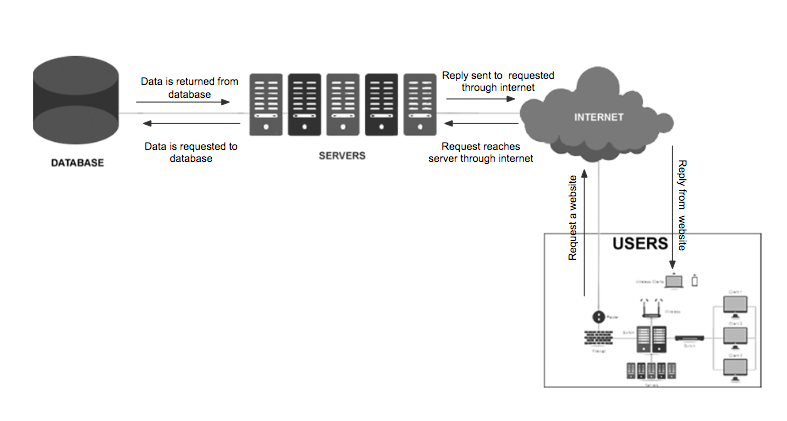
\includegraphics[width=15cm,height=10cm,keepaspectratio]{existing.png}
      \caption{Existing Methodology}
    \label{fig:Existing Methodology}
    
\end{figure}
A web server is a computer system that processes requesting is done via HTTP, which is used to distribute information on the World Wide Web. The term Webserver can refer to the entire system, or specifically to the software that accepts and supervises the HTTP requests.
\\

\hspace{5mm}A user or agent initiates communication by making a request for a specific resource using HTTP and the server responds with the content of that resource or if unable to do so with a error message. The resource can be a real file on the secondary storage of server,but this not necessarly depend on file type and depends on how the web server is implemented.
\\

\hspace{5mm}While the primary function is to serve content, a full implementation of HTTP also includes ways of receiving content from clients. This feature is used for submitting web forms, including uploading of files.
\\

\hspace{5mm}Many generic web servers also support server side scripting using Active Server Pages and PHP, or other scripting languages. This means that the behaviour of the web server can be scripted in separate files, while the actual server software remains unchanged. Usually, this function is used to generate HTML documents dynamically ("on-the-fly") as opposed to returning static documents. The former is primarily used for retrieving and/or modifying information from databases. The latter is typically much faster and more easily cached but cannot deliver dynamic content.
\\

\hspace{5mm}Web servers are not genarally used for serving the World Wide Web. They are also be found embedded in devices like printers,webcams,routers and serving only a local network. The web server may then be used as a part of a system for monitoring and/or administering the device in question. This usually means that no additional software has to be installed on the client computer, since only a web browser is required (which now is included with most operating systems).
\\

\hspace{5mm}Server-Client systems are today most frequently implemented by the request–response model: a client can send a request to the server,which performs the action and sends some response back to the client, typically with a acknowledgement or result. Designating a computer as "class-server hardware" implies that it is specialized for running servers on it. This often implies that it is more powerful and reliable than standard personal computers, but alternatively, large computing clusters may be composed of many relatively simple, replaceable server components.
\\
\newpage

\subsection{Proposed Methodology}\vspace{5mm}
\begin{figure}[ht!]
    \centering
    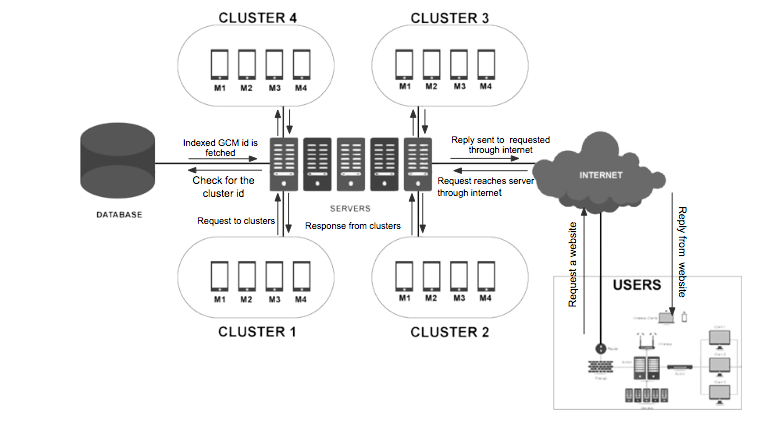
\includegraphics[width=18cm,height=15cm,keepaspectratio]{proposed.png}
     \caption{Proposed Methodology}
    \label{fig:Proposed Methodology}
\end{figure}
The model consists of servers, database, users and clusters of Mobile Data Servers. The operations are mainly controlled by the servers.The servers are linked to the clusters. Each cluster is a set of mobile phones, that are our MDS. Data is stored in these MDS and retrieved by the server as and when required.The interaction between with the users and servers, as well as the server and clusters takes place through the internet.\\

\subsubsection{Users}
User agent commonly a web browser initiate communication by making request for a specific resource using http. This request forwards to the application server. The users view a login page which act as a user authentication process and after login a file browser is viewed which can upload, view, download and delete the files. The  users can use the dropzone drag and drop method to upload the files or use the normal file upload method. The download is done by clicking a link which initiates the download action.  
\subsubsection{Application Server}
After receiving the request server searches the database and choose the mobile phones from the clusters in which the requested data is stored. The mobile phones communicate to the application server using the web services. The server communicate to the mobile phones using both Google Cloud Messaging services and web services. The application server also communicate with the database and maintain the records of the mobile phones and files that are sent to various mobile phones. The application server is responsible for securely processing the uploaded files and send it to various mobile phones. 
 \subsubsection{Database}
The database in the application server have the details of the mobile phones that are storing the requested data. It also have the details of the registered users and mobile phones . We are using MySQL Relational Database Management System for the Application Server as it is one of the easiest and open source program. We are using NoSQL database in Android for faster read and write capabilities of NoSQL compared to the SQLite in Android .
 \subsubsection{Android Systems}
 The encrypted data is splitted into different parts and each individual part of the data is saved in various android systems using snappyDB.Redundancy is also provided to maintain the consistency of the system.
\newpage
\subsection{Data Flow Diagrams} 
\begin{center}
\begin{figure}[ht!]
    \centering
  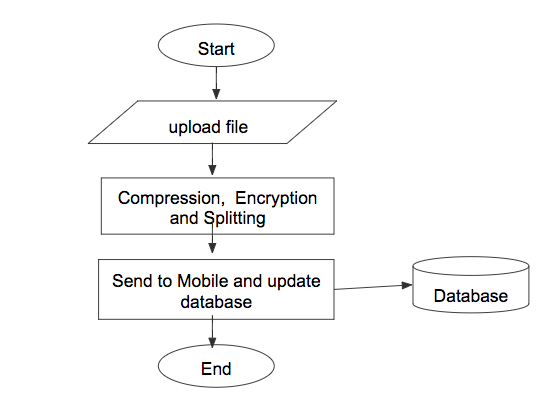
\includegraphics[width=15cm,height=6cm,keepaspectratio]{mdsnew.png}
    \caption{File Upload}
    \label{fig:File Upload}
\end{figure}

\end{center}
\vspace{-5mm}
The user agent can upload the file using filemanager,where he/she can upload,delete and download his files.Then the uploaded files will undergo compression and after that AES encryption is performed.This encrypted data is the splitted into different parts.Then each part of the encrypted data is stored in the mobile database,also the details of mobile phones in which each datapart is saved is maintained in the application server which makes the retrieval of data easier.

\begin{center}
\begin{figure}[ht!]
    \centering
    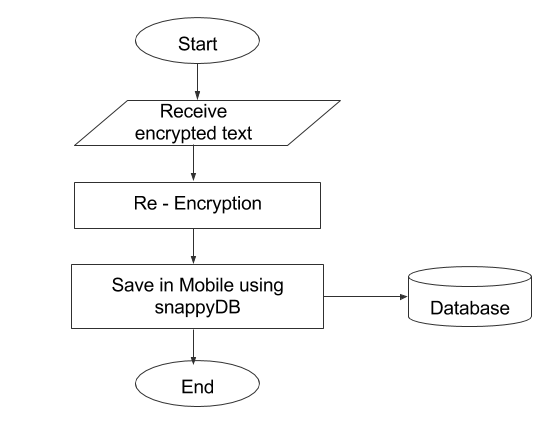
\includegraphics[width=15cm,height=6cm,keepaspectratio]{mdsnew1.png}
     \caption{Sending data to Android}
    \label{fig:Sending data to Android}
\end{figure}
\end{center}
After receiving the datapart in android systems it will undergo onemore AES encryption to provide additional security.Then the data will save in snappyDB of android systems.
\begin{center}
\begin{figure}[ht!]
    \centering
  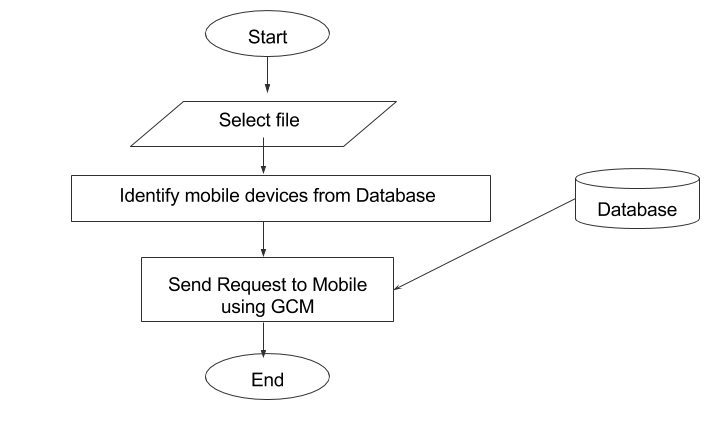
\includegraphics[width=15cm,height=6cm,keepaspectratio]{mdsnew2.png}
  \caption{Requesting the data}
    \label{fig:Requesting the data} 
    
\end{figure}
\end{center}
When a user request for a file ,from the application server the system can identify the android system in which the requested data is saved.Then inorder to check the liveness of mobile phones GCM service can be used.
\begin{center}
\begin{figure}[ht!]
    \centering
  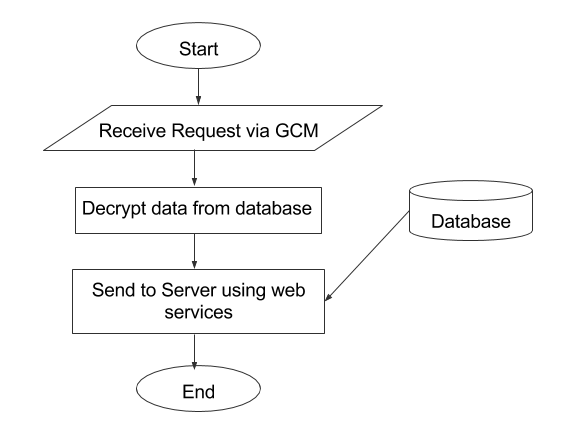
\includegraphics[width=15cm,height=6cm,keepaspectratio]{mdsnew3.png}
     \caption{Response from Android}
    \label{fig:Response from Android}
\end{figure}

\end{center}
After receiving the GCM request the corresponding mobile phone will respond to the server using webservices.first the requested data will undergo decryption and passes to the server.
\begin{center}
\begin{figure}[ht!]
    \centering
  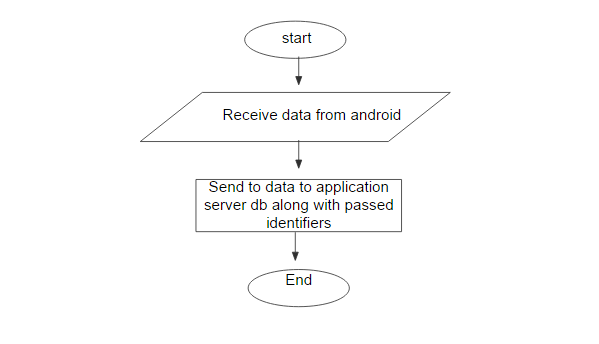
\includegraphics[width=15cm,height=6cm,keepaspectratio]{mdsnew4.png}
     \caption{Fetching the requested data}
    \label{fig:Fetching the requested data}
\end{figure}
\end{center}
After receiving the data from android systems it will forward to application server database.
\begin{center}
\begin{figure}[ht!]
    \centering
    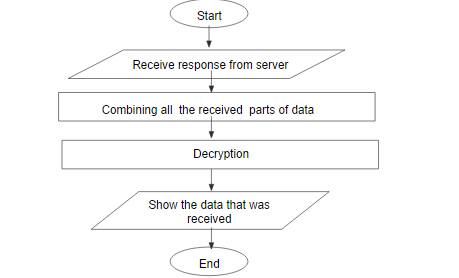
\includegraphics[width=15cm,height=6cm,keepaspectratio]{mdsnew5.png}
     \caption{Display the requested file}
    \label{fig:Display the requested file}
\end{figure}
\end{center}
After receiving the requested data,combine the different pieces which are received from different android systems and the entire file is shown to the requested user.

\newpage
\subsection{Technologies Used}\vspace{5mm}
\subsubsection{Server Side	}

\setenumerate[1]{label=\thesubsubsection.\arabic*.}
\setenumerate[2]{label*=\arabic*.}
\begin{enumerate}[leftmargin=1.5cm]
\item \textbf{PHP}\\PHP is a server scripting language, and a powerful tool for making dynamic and interactive Web pages.
PHP is a widely-used, free, and efficient alternative to competitors such as Microsoft's ASP.
The PHP Hypertext Preprocessor (PHP) is a programming language that allows web developers to create dynamic content that interacts with databases. PHP is basically used for developing web based software applications
\item \textbf{AJAX}\\AJAX is an acronym for Asynchronous JavaScript and XML. It is a group of inter-related technologies like JavaScript, DOM, XML, HTML, CSS etc.
AJAX allows to send and receive data asynchronously without reloading the web page. So it is fast.AJAX allows to send only important information to the server not the entire page. So only valuable data from the client side is routed to the server side. It makes your application interactive and faster.
\item \textbf{Web Services}\\A web service is any piece of software that makes itself available over the internet and uses a standardized XML messaging system. XML is used to encode all communications to a web service.Web services are self-contained, modular, distributed, dynamic applications that can be described, published, located, or invoked over the network to create products, processes, and supply chains. These applications can be local, distributed, or web-based. Web services are built on top of open standards such as TCP/IP, HTTP, Java, HTML, and XML.
\item \textbf{Google Cloud Messaging Service}\\Google Cloud messaging (commonly mentioned as GCM ) is a mobile notification service developed by Google that allows third-party application developers to send notifications, information or data from developer-run servers to applications that focus on the Google android OS, It also enables the applications or extensions developed for the Google Chrome web browser to send notifications. it's offered to developers free of cost.
\item \textbf{AES 256 bit Encryption}\\The Advanced Encryption Standard or AES is one of the symmetric block cipher which is used by the U.S. government and US Military to guard classified data . It is enforced in many software system and hardwares around the world to encrypt the  sensitive information.
\item \textbf{MySQL}\\MySQL  is an open source project based on Relational Database Management System (RDBMS). The MySQL development project made its source code and offered it under GNU General Public License. MySQL is owned  and supported by  the Swedish company MySQL AB, currently owned  by Oracle Corporation. For proprietary use, many paid editions are available.
\end{enumerate}
\subsubsection{Android Side}

\setenumerate[1]{label=\thesubsubsection.\arabic*.}
\setenumerate[2]{label*=\arabic*.}
\begin{enumerate}[leftmargin=1.5cm]
\item \textbf{Android}\\Android is a mobile OS developed by Google, that is developed based on the Linux
kernel and it's designed primarily for touch screen mobile devices like smartphones and tablets. Android’s UI relies on direct manipulation, using touch gestures that loosely correspond to  actions, like swiping, sound and pinching beside a virtual keyboard for text input. 
\item \textbf{Google Cloud Messaging Service}\\Google Cloud messaging (commonly mentioned as GCM ) is a mobile notification service developed by Google that allows third-party application developers to send notifications, information or data from developer-run servers to applications that focus on the Google android OS, It also enables the applications or extensions developed for the Google Chrome web browser to send notifications. it's offered to developers free of cost.
\item \textbf{SnappyDB}\\SnappyDB is a key-value based NoSQL database for android. It's an alternative database to  SQLite if you wish to use a NoSQL approach.It permits you to store and find primitive types, but also a Serializable object or array in a type-safe approach.SnappyDB will outmatch SQLite in read/write operations.
\item \textbf{AES 256 bit Encryption}\\The Advanced Encryption Standard or AES is one of the symmetric block cipher which is used by the U.S. government and US Military to guard classified data. It is enforced in many software system and hardwares around the world to encrypt the  sensitive information.
\end{enumerate}
\newpage
\begin{center}
\section{IMPLEMENTATION}
\end{center} 
Implementation is the stage of the project when the theoretical design is turned out into a working system. Thus it can be considered to be the most critical stage in achieving a successful new system and in giving the user, confidence that the new system will work and be effective.
The project implements PHP, Ajax, MySQL and standard HTML. The project will be capable of running on standard internet web browsers, although, the project is designed primarily around Google Chrome.
\subsection{Experimental Environment}
\subsubsection{Hardware Requirements}
\begin{itemize}
\item Android device with firmware v4.0(IceCream Sandwich) or above 
\end{itemize}
 
\begin{itemize}
\item Processor Pentium 4 or above
\end{itemize}
\begin{itemize}
\item RAM 1GB
\end{itemize}
\begin{itemize}
\item Hard disk 80GB
\end{itemize}
\subsubsection{Software Requirements}
\begin{itemize}
\item Operating System LINUX
\end{itemize}
\begin{itemize}
\item Front end HTML,CSS,AJAX
\end{itemize}
\begin{itemize}
\item Back end MySQL, PHP, AJAX
\end{itemize}
\begin{itemize}
\item Technology used: IDE Android Studio 1.0.1, Text Editor
\end{itemize}
\begin{itemize}
\item Emulators: Android Emulator
\end{itemize}
\begin{itemize}
\item Online Server Package - Apache shared server
\end{itemize}
\begin{itemize}
\item Tools used - Android SDK
\end{itemize}
\subsection{Implementation Explanations}
The project has a filemanager userinterface for  uploading the files inorder to use our service.He/she can delete and/or download the uploaded contents.The project is mainly divided into two modules a Web module and an App module. The web module controlls the flow of data and App module provides the storage space for the data.The app store the data in each mobile and act as a data base to main server.
\subsection{Evaluation Measures}

\newpage
\newpage
\begin{center}
\section{EXPERIMENTAL RESULTS}
\end{center}
\subsection{Dataset Description}

\subsection{Result Analysis}
\newpage
\begin{center}
\section{CONCLUSION and FUTURE WORK}
\end{center}  
   Creation and maintenance of large servers faces a lot of difficulties. An ideal server should function well irrespective of the amount of data it contained.In a server,the noticed problems are storage of data, resource shortage, pollution, massive power usage, cost to add new servers and latency issues.
So our proposed system will solve these issues.
\\

\hspace{5mm}For this, we utilize the storage resources of mobile devices so that the data must be stored in a distributed manner and can be accessed through an android application, thereby considerably reducing the number of existing servers. Due to these reduction in number, the existing servers can be efficiently utilized. Also power consumption is low and rate of pollution will be less.
 \\
 
\hspace{5mm}This model can be implemented on any android devices around the world and we can solve storage limitation. The mobile data servers are co-ordinated by a central server. The user query a data into the central server and it is fetched from the respective mobile device by the central server. The overall functioning of the system will be in a secure manner where we are using double encryption inside.
 \\
 
 \hspace{5mm}Since we are having billions of available mobile phones,this system is efficiently scalable.A less storage space of a single mobile phone is being part of large system.Simlilarly the storage from all the mobile phones will results in a huge storage space.So if this system is implemented,the issues related with data servers can be resolved and can replace the existing model of data retrieval through web sites.
\newpage
\begin{center}
\section{BIBLIOGRAPHY}\vspace{5mm}
\end{center}
\justify
\begin{enumerate}[label={[\arabic*]}]
\item \textbf{Seth Y.Fiawoo and Robert A.Sowah}, Department of Computer Engineering,University  of Ghana,\textbf{”Design and Development of an Android Application to Process and Display Summarised   Corporate Data”},  IEEE  4th International Conference on Adaptive Science and Technology(ICAST),2012
\item \textbf{Dimitris Economou, Suzanne Rivoire, Christos Kozyrakis} Department of Electrical Engineering Stanford University Partha Ranganathan,Internet Systems and Storage Lab Hewlett-Packard Labs,.\textbf{”Full-System Power Analysis and Modeling for Server Environment”}
\item \textbf{D. Roselin Selvarani},  Department of Computer Science, Holy    Cross College, Bharathidasan University, Tamil Nadu, India and  Dr. T.N. Ravi, Department of Computer Science, Periyar    E.V.R. College, Bharathidasan University,  Tamil Nadu, India.\textbf{“A Review on the role of Encryption in Mobile Database Security”}, International Journal on Application or Innovation  in Engineering and Management, December 2014
\item \textbf{Wumuti Naheman,} College of Resources and Environment Sciences Xinjiang University Urumqi, China and Jianxinwei,  Information Center of Xinjia Land Resources Department Urumqi,China , \textbf{ ”Review of NoSQL Databases and Performance Testing on HBase” }, International Conference on Mechatronic Sciences, Electric Engineering and Computer (MEC), Shenyang, China, 2013
\item \textbf{Moussa Demba,} Department of Computer Science \& Information, Aljouf University Sakaka, Kingdom of Saudi Arabia \textbf{“Algorithm for Relational Database Normalization up to 3NF”}, International Journal of Database Management Systems ( IJDMS ) Vol.5, No.3, June 2013
\item \textbf{Ibikunle},Electrical and Information Department, Covenant University, Nigeria and \textbf{Adegbenjo},Computer Science Department, Babcock University, Nigeria,
\textbf{“Management Issues and Challenges in Mobile Database System”}, International journal of Engineering Sciences and Emerging Technologies, April 2013
\item \textbf{Vishnu Swaroop and Udai Shanker},Department of Computer Science \& Engineering, M.M.M. Engineering College, Gorakhpur
\textbf{“Data management in Mobile Distributed Real Time Database Systems: Reviews and Issues”}
 International Journal of Computer Science and Information Technologies(IJCSIT), Vol. 2(4),   2011, 1517-1522
 \item \textbf{Hongli Su,} Liaoning Finance Vocational College,”\textbf{The Processing Technology in Mobile Database Transaction System”},  International Journal of Database Theory and Application Vol.8, No.2 (2015), pp.51-60
\item \textbf{Yishan Li,} University of Auckland and \textbf{Sathiamoorthy Manoharan}, \textbf{“A Performance Comparison of SQL and NoSQL databases”}, IEEE Pacific Rim Conference on Communications, Computers and Signal Processing(PACRIM), 2013
\item \textbf{Suhas Holla and Mahima M Katti},Department of Information Science \& Engg, R V College of Engineering Bangalore, India
\textbf{“Android based mobile application devolopment and its security”}
 International Journal of Computer Trends and Technology- volume3,Issue3- 2012
 \item \textbf{Kundankumar Rameshwar Saraf, Vishal Prakash Jagtap and Amit Kumar Mishra },Department of Electronics and Telecommunication Engineering Sandip Institute of Technology and Research Centre, Nasik, Maharashtra
\textbf{“Text and Image Encryption Decryption Using Advanced Encryption Standard ”}
International Journal of Emerging Trends \& Technology in Computer Science (IJETTCS),
Volume 3, Issue 3, May – June 20
\item \textbf{Divya Singh, Pragun Arora Rakshit and Saket Tomar},Department of Computer Science and Engineering, AMITY University Greater Noida, Scholar, Department of Computer Engineering, AMITY University Greater Noida
\textbf{“Study of Data Transmission Using socket”}
 International Journal of Computer Science and Mobile Applications, Vol.2 Issue. 11, November- 2014, pg. 150-154
\item \textbf{https://developer.android.com} - Android Developer Manual ,  Android provides a rich application framework that allows you to build innovative apps and games for mobile devices in a Java language environment. The documents listed in the left navigation provide details about how to build apps using Android's various APIs.
\item \textbf{http://www.snappydb.com} - Snappy DB Developer Manual , SnappyDB is a key-value database for Android it's an alternative for SQLite if you want to use a NoSQL approach.It allows you to store and get primitive types, but also a Serializable object or array in a type-safe way.SnappyDB can outperform SQLite in read/write operations.
\item \textbf{https://www.tutorialspoint.com/webservices} - Web services are open standard (XML, SOAP, HTTP etc.) based Web applications that interact with other web applications for the purpose of exchanging data.Web Services can convert existing applications into Web-applications.
\end{enumerate}

